
% this file is called up by thesis.tex
% content in this file will be fed into the main document

%: ----------------------- introduction file header -----------------------
% the code below specifies where the figures are stored
\graphicspath{{5/figures/}}

\chapter{Automatic Chord Estimation}
\label{chp:chord_estimation}

\section{Context}
\label{sec:context}

% Timbre, though hard to define, is relatively constrained
Though a satisfactory definition remains elusive, it is important to recognize that the perception of timbre is tightly coupled with its physical acoustic stimulus.
Similar to the perception of pitch or loudness, all information necessary to model human experience is contained within the signal representation.
These kinds of low-level percepts are literal in nature, especially when compared to more abstract concepts like artist recognition or estimating tension.
As it is a particular goal of this work to explore how deep learning methods can be applied to the murky waters of music analysis, we now turn our attention to the problem of automatically transcribing chords from polyphonic music recordings.

\subsection{Musical Foundations}
\label{subsec:musical_foundations}

In lieu of a general, perhaps impossible, definition of ``music'', we instead arrive at a confined concept through a set of constraints.
Here, we are primarily interested in the tradition of tonal Western music, with a particular focus on popular contemporary music from the last century, built upon a 12-Tone Equal Temperament (12-TET) tuning system.
Furthermore, music typically lives in two domains: one, \emph{symbolic}, in the form of scores, MIDI, or countless other forms of abstract musical representations; and two, rendered via synthesis as \emph{sound signals}, which may be transmitted through physical space as acoustic waves or stored in a persistent state as static information, e.g. a sound recording.
% Framed in this way, this work is concerned with the machine audition of music, whereby sound signals are transformed into some form of symbolic notation.

% Dimensions of music
Continuing, it can be said that there are three fundamental dimensions to this kind of music:

\begin{itemize}
\item Rhythm: the understanding of loudness as a function of time.
\item Harmony: the understanding of pitch as a function of time.
\item Timbre: the understanding of sources as a function of time.
\end{itemize}

In all three dimensions, observable signal qualities give rise to sensory percepts.
``Loudness'' is defined as the phenomena whereby sound stimuli can be compared with respect to intensity, and is closely related to signal power.
Orthogonally, ``pitch'' is defined as the phenomena whereby a sound stimulus can be matched to the frequency of a pure sinusoid, and is a result of the harmonic components, or partials, found in complex sounds.
Lastly, and in spite of timbre's ambiguous nature, we constrain it here to mean the phenomena by which concurrent voices may be identified and differentiated in a single sound stimulus.

% Historical context -> Harmonic analysis
Contextualizing briefly, theorists have long sought to characterize musical works via analysis and reduction as a means to understanding.
With sound recording being a relatively modern invention on the timescale of music history, much effort to this end has been invested in the analysis of symbolic notation, or scores.
%, which cleanly delineate the three dimensions described previously; an example of this is given in Figure \ref{fig:notated_music}.
Evolving over time from the counterpoint of J. S. Bach to the functional analysis of Heinrich Schenker or more recently Fred Lehrdal, traditional musical analysis revolves heavily around the harmonic facets of a musical piece by marginalizing the dimensions of rhythm and timbre.
As a result, the harmonic language of ``chords'' developed as a rich yet compact vocabulary to describe a piece of music; an instance of such a harmonic analysis is given in Figure \ref{fig:notated_music}.

% Attempts to define a chord
Unfortunately, what comprises a chord is open to some interpretation, and no singular definition exists.
For example, \cite{McVicar2013} collects three possible definitions of a chord, restated here:

\begin{enumerate}
\item \emph{Everyone agrees that \emph{chord} is used for a group of musical tones.}
\item \emph{Two or more notes sounding simultaneously are known as a chord.}
\item \emph{Three or more pitches sounded simultaneously or functioning as if sounded simultaneously.}
\end{enumerate}

% Pitch and notes
Alternatively, \cite{Harte2010} expands the scope of (2) in order to describe a wider space of music, ``allow[ing] a chord to comprise zero or more notes.''
It is both important and interesting to observe the concepts of \emph{pitch}, \emph{tone}, and \emph{note} are used interchangeably.
For clarity, a tone is a perceptual object with a pitch, whereas a note is a musical object that may be realized as sound subject to a given tuning system.
The relationship between the two in equal temperament is defined as the following:

\begin{equation}
\label{eq:tuning}
f_{pitch} = f_{tuning} * 2 \exp((n_{index} - 48) / N)
\end{equation}

\noindent~where $N$ is the number of notes per octave, $n_{index}$ is an integer note index, $f_{tuning}$ is the frequency, in Hertz, of a reference tone, and $f_{pitch}$ is the resulting frequency, in Hertz, of the corresponding note.
An \emph{octave} is defined as the doubling of a quantity, and exhibits a special relationship in human perception by which two tones, differeing by an integer power of 2, are perceived as similar; this phenomena is referred to as octave equivalence \cite{?}.

Therefore, in 12-TET, it is useful to name the unique pitch classes per octave, given in the following ordered set, $\mathcal{P}$:

\begin{equation}
\label{eq:pitch_classes}
\mathcal{P} = \{C, C\sharp / D\flat, D, D\sharp / E\flat, E, F, F\sharp / G\flat, G, G\sharp / A\flat, A, A\sharp / B\flat, B\}
\end{equation}

An absolute note name, consisting of a pitch class and an octave index, is given by the following as a function of absolute note index, such that $n_{index}=0~\to~C0$:

\begin{equation}
(\mathcal{P}[mod(n_{index}, 12)], \lfloor~n_{index} / 12~\rfloor)
\end{equation}

In contemporary music, standard concert tuning equates $A4=440Hz$; classically, the tuning frequency is defined such that it falls in the performance range of a majority of instruments to be matched exactly, and hence the offset in Eq. \ref{eq:tuning}.
Were this tuning frequency constant, the notions of pitch and note would be equivalent; it should be noted, however, this is not always the case.

% Chord composition
It may be difficult or ambiguous to infer the significance of a pitch collection by notes alone, and therefore chords are typically named according to three criteria: the relative intervals between the notes it contains, the note corresponding to the \emph{root}, and its overall relationship to the local \emph{key}.
Intervals describe the integer distance between notes: adjacent notes or pitch classes is referred to as a \emph{semitone}, with a step size of 1, whereas a step size of 2 is known as a \emph{whole tone}.
A ``root'' is the note in a chord that serves as a point of \emph{internal} harmonic stability; conversely, a ``key'' is itself a chord which serves as a point of \emph{external} harmonic stability.
Therefore, as we will shortly see, the name a chord takes can change based solely on contextual information.

% Chord Names
The final piece of information necessary before we can discuss chord spellings is the concept of the diatonic scale, upon which the vast majority of Western harmony is built.
It is expressed here as an ordered set of intervals ($T$ for whole tone, $s$ for semitone) and relative semitone degrees:

\begin{equation}
\mathcal{D}_{intervals} = \{T, T, s, T, T, T, s\} \\
\mathcal{D}_{semitones} = \{0, 2, 4, 5, 7, 9, 11\}
\end{equation}

\noindent Using the diatonic scale to index a set of pitch classes in \ref{eq:pitch_classes}, one arrives at a \emph{major} scale, where the starting note is referred to as the \emph{tonic}.
In the key of $C$, this takes the following form:

\begin{equation}
\mathcal{C}_{major} = \{C, D, E, F, G, A, B\}
\end{equation}

We can now build our first chord \emph{quality}, the major triad, comprised of the first, third, and fifth major scale degrees:

\begin{equation}
\mathcal{M}_{semitones} = \{0, 4, 7\} \\
\text{e.g. in the key of} C, C:maj = \{C, E, G\}
\end{equation}

Note that a triad is any chord comprised of three notes; later, we will also consider tetrads, or chords consisting of four notes.
Additionaly, we introduce the concept of a quality here to describe the root-invariant components of a chord, i.e. the intervals.

Rotating the diatonic scale produces other \emph{modes}, of which the most common is minor, resulting from a circular shift of 3:

\begin{equation}
\mathcal{m}_{intervals} = \{T, s, T, T, s, T, T\} \\
\mathcal{m}_{semitones} = \{0, 2, 3, 5, 7, 8, 10\}
\end{equation}

\noindent Starting this time from $A$, we arrive at the resulting minor scale:

\begin{equation}
\mathcal{A}_{minor} = \{A, B, C, D, E, F, G\}
\end{equation}

We can now build our second chord \emph{quality}, the minor triad, comprised of the first, third, and fifth \emph{minor} scale degrees:

\begin{equation}
\mathcal{m}_{semitones} = \{0, 3, 7\} \\
\text{e.g. in the key of} A,~A:min = \{A, C, E\}
\end{equation}

% Chord Observations
Here, a few important observations should be made.
First, the scales of $\mathcal{C}_{major}$ and $\mathcal{A}_{minor}$ are comprised of the exact same pitch classes, differing only as a function of where the scale begins; these are known as relative major and minor scales, respectively.
Additionally, a triad can be formed taking any scale degree as its root, and as a result different keys will share chords.

% Why is it so hard to define a chord? Let's look at some examples
Having covered the basic elements of Western tonal theory, it is now possible to develop a better understanding of the variation and difficulty in defining a chord by exploring a few specific, if simple, examples.
The one invariant property shared by all defintions named previously is the idea that a pitch collection may be understood as a single entity.
The time span over which this phenomena may unfold, however, is flexible.
To illustrate the point, consider the three bars notated in Figure \ref{fig:expanded_major}, where a major chord is written as a true simultaneity, an arpeggiation, and as an series of non-overlapping quarter notes, respectively.
In this instance, the degree of overlap in time is expanded until it no longer exists, and yet the collection of notes continues to function as a coherent harmonic object.

\begin{figure}[t]
\centering
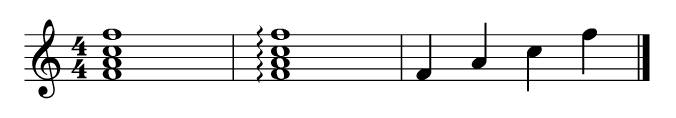
\includegraphics[width=5in]{expanded_major}
\caption{writeme}
\label{fig:expanded_major}
\end{figure}

On the other hand, as shown in Figure \ref{fig:nonchord_tones}, the simultaneous sounding of different notes does not necessarily give rise to the perception of different chords.
Here, a major triad is sustained under the first several degrees of its scale.
While three notes in the upper voice are contained in the C:maj triad, the other three --the D, F, and A-- are known as ``nonchord'' tones.
These ``extra'' tones, however, can be explained away in the overall harmonic scene, as they fall on metrically weak beats, are comparatively short in duration, and are quickly resolved to chord tones.
As a result, they do not contribute significantly to the harmonic center of the phrase, and the bar is still understood as a stable C:maj.


\begin{figure}[t]
\centering
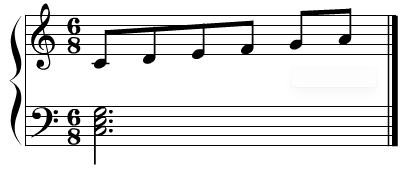
\includegraphics[width=3in]{nonchord_tones}
\caption{writeme}
\label{fig:nonchord_tones}
\end{figure}

A final example, shown in Figure \ref{fig:fifths_context}, demonstrates the role that context and the perception of key can play on the understanding of a chord.
Here, two diatonic scales --one major and the other minor-- descend to identical pitch combinations, consisting of the tonic, fifth, and octave degrees.
Therefore, even though the chords are absent a third scale degree, they are perceived as having the quality of the leading context, being major and minor respectively.
Though similar in principle to that of Figure \ref{fig:expanded_major}, this example serves to demonstrate that ambiguous simultaneities can be resolved by incorporating contextual information.

% Real music on the other hand, like the first system of a Beethoven string quartet given in Figure \ref{fig:beethoven}, can be remarkably complex and require a good deal of expertise to complete a formal analysis of the score.
% Skilled musicans are quite robust in the ability to assign chord labels to musical scenes despite an occasionally opaque decision making process, and it is an exciting challenge to produce a computational system with a similar capacity.
% However, as discussed in the following section, the topic is also motivated by a long research tradition in MIR.

% \begin{figure}[!t]
% \centering
% 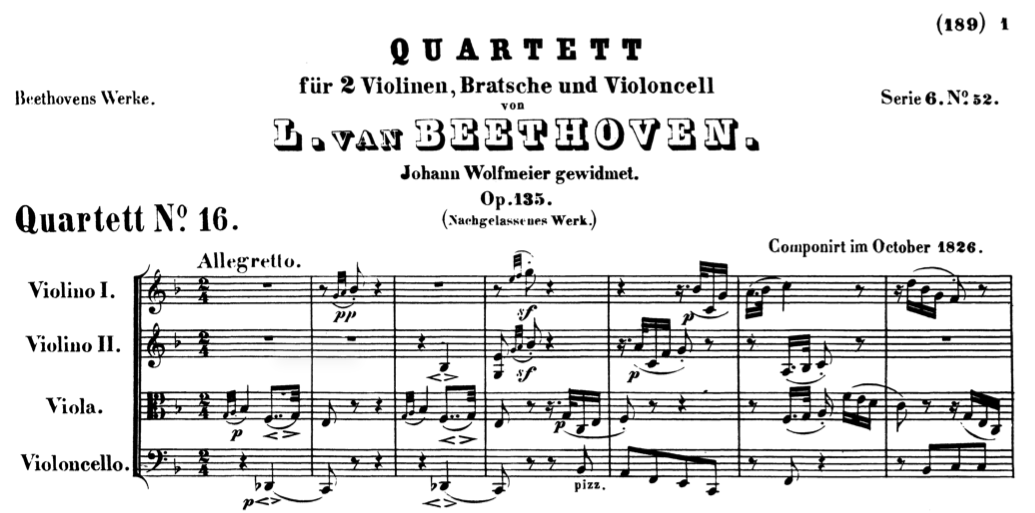
\includegraphics[width=5in]{beethoven}
% \caption{writeme}
% \label{fig:beethoven}
% \end{figure}

\subsection{Chord Syntax}
\label{sec:chord_syntax}

It is a pragmatic but ultimately necessary prerquisite step to define a standard syntax for consistently referencing and describing chords.
Much of the pioneering work in this space was performed by Harte \cite{Harte2010}, and many of these conventions are utilized here.
For clarity, we stylize chords in this syntax with a fixed-width font, e.g. \texttt{A:min}.

Firstly, Harte's general chord notation is described by the following four-part symbolic description:

\begin{equation}
\{r\}:\{q\}(i)/\{b\}
\end{equation}

\noindent Every chord name begins with a root $r$ in the form of a valid pitch class, optionally modified by zero or more sharps or flats, or one of two reserved characters: \texttt{N} for the ``null'' no-chord condition, or \texttt{X} for the special case in which the musical content cannot be described harmonically.

The root name is potentially followed by a quality shorthand, $q$, separated by a colon and implying a particular set of note intervals.
Though there are a large number of possible chord qualities, this is often limited to a particular subset in practice.
Those considered in this work are indicated in the following table:

\begin{table}[h]
\begin{center}
\caption{Chord quality names and corresponding relative semitones.}
\begin{tabular}{l | c | c}
Name & Shorthand & Semitones \\
\hline
Major & \texttt{maj} & $\{0, 4, 7\}$ \\
Minor & \texttt{min} & $\{0, 3, 7\}$ \\
Major 7 & \texttt{maj7} & $\{0, 4, 7, 11\}$ \\
Minor 7 & \texttt{min7} & $\{0, 3, 7, 10\}$ \\
Dominant 7 & \texttt{7} & $\{0, 4, 7, 10\}$ \\
Major 6 & \texttt{maj6} & $\{0, 4, 7, 9\}$ \\
Minor 6 & \texttt{min6} & $\{0, 3, 7, 9\}$ \\
Diminished & \texttt{dim} & $\{0, 3, 6\}$ \\
Augmented & \texttt{aug} & $\{0, 4, 8\}$ \\
Suspended 2$^{nd}$ & \texttt{sus2} & $\{0, 2, 7\}$ \\
Suspended 4$^{th}$ & \texttt{sus4} & $\{0, 5, 7\}$ \\
Fully-diminished 7 & \texttt{dim7} & $\{0, 3, 6, 9\}$ \\
Half-diminished 7 & \texttt{hdim7} & $\{0, 3, 6, 10\}$ \\
\hline
\end{tabular}
\label{tab:qualities}
\end{center}
\end{table}


The third field provides an interval set, $i$, wrapped by parentheses.
In practice, there are two reasons for representing information intervallically.
One such instance is, through a combination of additional degrees and asterisks, the modification of a quality shorthand in order to represent a non-standard, but related, chord.
An example of this might be the chord name \texttt{A:min(\*b3, 7)}, which means that the minor third ($C$) is absent, but a major 7 ($A\flat$) has been added.
The other instance occurs when the intervals are certain but the quality is ambiguous, such as \texttt{C:(1, 5)}; note that this is a valid spelling of the chord shown in Figure \ref{fig:powerchord_context}.

The final field of this chord syntax is the bass interval, $b$, which indicates the scale degree at the bottom of the chord.
Typically this is also the root of the chord, and is implied in the absence of an explicit bass interval.
However, it is necessary to state that the scale degrees of the chord --given by the quality shorthand and the interval set-- can be further augmented by the inclusion of a bass interval.
For example, the chords \texttt{C:maj/b7} and \texttt{C:7} would be understood as containing the same pitch classes, but are spelled quite differently.


\subsection{Motivation}
\label{subsec:motivation}

% Historical Context
Even from the earliest efforts in content-based music informatics research, automatic music transcription has stood as one of the Holy Grails of the field.
Over time, however, it would prove exceptionally difficult, and fracture into a variety of smaller, and hopefully more manageable, subtopics.
As a result, automatic chord estimation materialized as one such task, now receiving healthy attention for more than a decade, and established as a benchmark challenge at the annual MIReX event \footnote{{http://www.music-ir.org/mirex/wiki/MIREX\_HOME}}.

% Applications
% - People
Given the prerequisite skill necessary to produce these transcriptions manually, there is considerable motivation to develop automated systems capable of reliably performing this task.
As evidenced by large online communities surrounding websites like e-chords\footnote{http://www.e-chords.com} or Ultimate Guitar\footnote{http://www.ultimate-guitar.com}, countless individuals invest considerable time and effort in the curation and consumption of popular music transcriptions.
Often this is driven by desire to learn and perform music for which symbolic notation does not exist.
Conversely, automatic chord transcription systems would be particularly useful in the areas of composition, recording, and production.
Furthermore, the curation of this content would enable large-scale musicological analysis of contemporary music.

% MIR Systems
In addition to the concerns of individual users, computational systems capable of reliable chord transcription are directly useful inside the domain of content-based MIR.
Chords can serve as a robust mid-level representation with which to build systems and extract higher level musical knowledge.
This has been used in the space of cover song retrieval \cite{Juan?}, navigating large collections \cite{alan?}, and genre recognition \cite{anglade}.
Such systems would also facilitate data collection for other tasks, aiding in visualization and other facets of music transcription.

% Theoretical merit
From a more philosophical perspective, the identification of chords is also intriguing as an intelligent musical behavior, being a high level cognitive process that is often open to multiple interpretations between knowledgable experts.
Experiential bias of the annotator may manifest in the subjective decisions made by an observer, where a pianist may arrive at a different harmonic analysis than that of a guitarist due to how a collection of notes might be produced.
Lastly, the knowledge and skill of the one recognizing chords in music will affect the resulting interpretations.
Beginners will likely prefer simple or more common descriptions, whereas experts will be more aware of complex nuances and have better command over a larger harmonic vocabulary.


\subsection{Limitations}
\label{subsec:limitations}
% Limitations
It should be acknowledged that such an inquiry is subject to certain limitations, and there are two worth mentioning here.
The first derives from the philosophical limits of objective truth in an inherently subjective task.
As outlined previously, the definition of a chord is open to interpretation, and may be influenced by individual experience, degree of skill, and intended purpose.
This begs a potentially damning question: What hope is there for an automatic algorithm if you can't define your concepts?
Furthermore, ``expert'' annotations used in the development and evaluation of computational systems is based on the assumption that all subjects apply the same rules to some unknown degree of consistency.

The second notable limitation is related to the validity and relevance of chords as a means to describe musical content.
Even in the constrained space of Western tonal music set forth here, not all musical works will be well-described by the language of harmonic analysis.
Therefore a chord transcription may be a poor approach toward representing such a piece of music.
In some cases an alternative approach to analysis, such as voice leading, might make more sense; in others, such as rap or math rock, a lack of clearly structured harmonic content may arguably render the goal of harmonic analysis altogether irrelevant.


\section{Previous Efforts in Automatic Chord Estimation}
\label{sec:background}

In this section, we attempt to develop a formal defintion of the automatic chord estimation task, and detail the standard methodology used by the research community.
We then close with a brief survey of the state of the art and the apparent trajectory of the research topic.


\subsection{Problem Formulation}
\label{subsec:problem_formulation}

% Problem formulation
Consistent with the motivations outlined in \ref{subsec:motivation}, the goal of an automatic chord estimation (ACE) system is --or, at least, has been-- to produce an objectively ``good'' time-aligned sequence of chords from a given music signal.
This established notion of objectivity is crucial to how the problem is approached, whereby conventional methodolgy prefers repeatable, quantitative evaluation as a proxy to qualitative feedback collected from human subjects.
While the latter is generally preferable to the former, such user studies can be prohibitively costly in both time and money to conduct with any regularity.
As a result, the research of computational systems that model human behavior often proceeds by collecting some number of input-output datapoints from human subjects \emph{beforehand}, and subsequently measuring the degree to which a system can produce these outputs from the inputs.
Importantly, this paradigm operates on the assumption that these human provided input-output pairs, conventionally referred to as ``ground truth'' in various domains, are absolute, and not a function subject.

% Datasets and human annotations
The first major effort to curate ground truth chord transcriptions was led by Harte in the mid-2000s \cite{Isophonics}, where a small team of individuals transcribed the entire discography of The Beatles.
Containing chord annotations for 180 tracks, this was a landmark dataset in the field of MIR and shaped years of ACE research.
More recently, two datasets were made publicly available following the 2011 Conference of the International Society of Music Information Retrieval (ISMIR), one of over 700 tracks led by J. Ashley Burgoyne \cite{Burgoyne2011} and another of 295 tracks led by Tae Min Cho \cite{Cho2011b}; for convenience, we will refer to the former as ``Billboard'' and the latter as ``NYU'', corresponding to the related projects.
Along the way, one additional, comparatively small, dataset was released, containing 20 tracks by the band Queen, provided by Matthias Mauch \cite{Mauch2009x}.
In all four cases, the chord transcriptions are provided on the premise that the data corresponds to the ``expert'' perspective.
To prevent errors or resolve judgment calls, all annotation efforts named above employed a review process, where the transcriptions of one or more annotator were verified by a different individual.

% Transcription, estimation and recognition
% Somewhat ironically, there is some inconsistency in the literature regarding what this task should be called.
% Mauch makes mention of this in his thesis \cite{Mauch2010PhD},

% The issue of vocabularies -- Major-minor Chord mapping
As we have seen in \ref{subsec:foundations}, it is a particular nuance of chord naming conventions that the vocabulary of possible chord names is effectively infinite.
This results in a few practical problems that must be resolved.
While the majority of musical content will be well described by a bounded subset of chord spellings, a large number of low-frequency chord names will naturally occur in a dataset.
This is made worse by the reality that some chord qualities, namely \texttt{maj} or \texttt{min}, are simply more common than the rest.
Taken together, chord estimation systems are typically designed to classify chords among a fixed vocabulary defined \emph{a priori}.

In the history of ACE, the choice of vocabulary has been anything but standard, influenced by a variety of factors.
Data-driven approaches, for example, can be sensitive to the amount of labeled data available to train a given model, in which case it might be advantageous to discard under-represented chord classes.
Alternatively, it might be a useful constraint of the system to only predict the most common chords, helping to cut down on confusions and spurious errors, or perhaps a researcher is not particularly interested in detecting inversions.
It therefore becomes equally challenging to compare the performance of systems designed for different vocabularies.

One common strategy devised by the community to cope with this variation is the concept of Major-Minor chord resolution.
This proceeds by taking the space of all chord names in a collection of transcribed music recordings, and mapping each chord name to either a Major or Minor chord with the same root \cite{McVicar2013}.
Though some chord quality resolutions are musically reasonable, e.g. \texttt{maj7} $\to$ \texttt{maj}, others are less sound, e.g. \texttt{dim7} $\to$ \texttt{min} or \texttt{aug} $\to$ \texttt{maj}.
A thorough discussion on the impacts of such decisions will take place in Section \ref{sec:pilot_study}, but we address the practice of \emph{vocabulary resolution} here to call attention to the fact that, save for a few exceptions, the majority of ACE research and methodology focuses on this artificial Major-Minor formulation.


\subsection{Computational Approaches}
\label{subsec:computational_approaches}

% Previous work
Historically speaking, nearly all approaches to the ACE task adopt the same basic architecture, diagrammed in Figure \ref{fig:basic_ace}.
First, harmonic features, referred to as pitch class profiles (PCP) or \emph{chroma}, are extracted from short-time observations of the audio signal.
Initially proposed for use in chord estimation systems by Fujishima \cite{fujishima1999}, chroma features attempt to measure the amount of energy in the signal corresponding to the 12 pitch classes named in Eq. \ref{eq:pitch_classes}.
These features may then be processed by any number of means, referred to in the literature as \emph{pre-filtering}.
Importantly, this is done prior to the next stage of \emph{pattern matching}, which is performed on the final feature representation to measure how similar the observed signal is to a set of chord names.
The process of pattern matching, a relatively local operation, is mapped over a much longer signal, e.g. a full recording, yielding a time-varying estimate of the various chord types the model can represent.
Finally, \emph{post-filtering} is applied to the output of the pattern matching stage, resulting in a sequence of chord names over time.

Though the implementation details have continued to evolve over the last decade, the brunt of chord estimation research has concentrated not on the fundamental system per se, but rather the tuning of its components.
In particular, much time and energy has been invested in developing not just better features, but specifically better \emph{chroma} features \cite{muller2010}.
Complementing chroma features, others have explored the use of multi-band chroma to model bass frequencies separately \cite{Mauch2009?} or a Tonnetz representation in an effort to better encode harmonic relationships between chords \cite{Lee2007}.
Acknowledging the challenges inherent to designing good features, Pachet et al pioneered work in automatic feature optimization \cite{pachet2004}, and more recently deep learning methods have been employed to learn robust Tonnetz features \cite{ejh2011}.
Early methods focused on local smoothing, such as low-pass \cite{} or median \cite{} filtering as a form of pre-filtering, but more recently some methods have attempted to leverage the repeated nature of music to yield more stable estimates of the harmonic composition at a given point in time \cite{Cho2011}.
Various classification strategies have been investigated such as binary templates \cite{?}, Dirichlet distribution models \cite{Burgoyne2008?}, or Support Vector Machines (SVMs) \cite{weller2009}, but Gaussian Mixture Models (GMM) are by and large the most common feature modeling approach \cite{a,b,c}.
The choice of post-filtering methods has been shown to significantly impact system performance, and much research has focused on properly tuning Hidden Markov Models (HMMs) \cite{Cho2010}, first introduced by \cite{sheh2003}.
Recently, in an effort to continue to advance the state of the art, researchers have begun exploring more complex post-filtering methods such as Dynamic Bayesian Networks (DBNs) \cite{mauch2010b, McVicar2013} and Conditional Random Fields (CRFs) \cite{?}.

It is worth noting that in this lineage, the systems that do make use of data-driven learning typically only do so in disjoint stages.
More often than not, machine learning is only performed at the pattern matching stage, where increasingly powerful models are fit to hand-crafted features.
A few works do attempt to learn features, such as \cite{MauchNNLS, Humphrey2012?}, but the different stages are optimized independetly.
Though it is standard practice to train a GMM/HMM jointly, some have observed that learning the parameters of the HMM, i.e. the transition probabilities, yields no significant benefit over a uniform probabilities with a strong self-transition affinity \cite{Cho2014PhD}.
One notable work that attempts to jointly optimize multiple stages is that of \cite{Kim2012}, which optimizes the GMM to a minimum classification error (MCE), rather than a conventional maximum likelihood formulation.


\subsection{Evaluation Metrics}
\label{subsec:evaluation_metrics}

We now formalize an approach to comparing, and subsequently scoring, the relative agreement between two chord transcriptions.
The classic metric reported in ACE research is conceptually some kind of total mutual agreement score, $S$, between a set of $N$ reference, $\mathcal{R}$, and estimated, $\mathcal{E}$, transcriptions as a continuous integral over time, defined by the following:

\begin{equation}
S_overall = \frac{1}{W}\sum_{n=0}^{N-1}\int_{t=0}^{T_n}C(\mathcal{R}_n(t), \mathcal{E}_n(t))\partial~t
\end{equation}

\noindent where $C$ is a chord comparison function, $t$ is time, $n$ the index of the track in a collection, $T_n$ the duration of the $n^{th}$ track, $W$ the cumulative amount of time on which $C$ is defined.
More explicitly, $W$ is computed by a similar integral:

\begin{equation}
W = \sum_{n=0}^{N-1}\int_{t=0}^{T_n}(\mathcal{R}_n(t), \mathcal{E}_n(t) \in \Re)\partial~t
\end{equation}

Defining the score normalization term $W$ separately is useful when comparing chord names, as it relaxes the assumption that the comparison function is defined for all possible chords.
Therefore vocabulary selection or resolution can be delayed until evalutation, and all emphasis can be placed on the comparison function $C$.
In practice, this measure is known as \emph{Total Correct Overlap} (TCO) \cite{Mauch, Harte, McVicar}, \emph{Weighted Chord Symbol Recall} (WCSR) \cite{MIReX}, or \emph{Framewise Recognition Rate} \cite{Cho2014}.
Effectively, this is a multiclass version of recall, which is expressed by the following:

\begin{equation}
r = \frac{true~positives}{all~positives}
\end{equation}

Precision, a complement to recall, can also be expressed similarly:

\begin{equation}
p = \frac{true~positives}{true~positives + false~positives}
\end{equation}

\noindent While the definition of recall intuitively extends to the multiclass condition faced in ACE, it is worthwhile to consider the meaning of precision.
In this instance, such a measure provides insight into how reliable the estimated chord name are.
For example, a system could heavily over-predict the most common chord labels to achieve a high recall value, but the precision might still be comparatively low.
% Notably, if the errors (false positives) are decorrelated, then recall and precision will converge to the same value.
Standard practice in information retrieval also considers the harmonic mean of these two metrics, known as the $f_1$ score, which captures both behaviors in a single measure:

\begin{equation}
f_1 = \frac{pr}{2(p+r)}
\end{equation}

Finally, it was recently proposed by Cho in \cite{Cho2014PhD} that, when working with larger chord vocabularies, special attention should be paid to performance across all chord qualities.
The motivation for additional measures stems from the reality that chord classes are not uniformly distributed, and a model that ignores infrequent chords will not be well characterized by global statistics.
This can be extended to the metrics above by adding a quality condition to the comparison function and averaging over qualities:

\begin{equation}
S_{quality\_ave} = \sum_{q=0}^{Q-1}\frac{1}{W_q}\sum_{n=0}^{N-1}\int_{t=0}^{T_n}C(\mathcal{R}_n(t), \mathcal{E}_n(t) | q)\partial~t
\end{equation}

\noindent Referred to as \emph{Average Chord Quality Accuracy} (ACQA), this is simply a recall measure where the contributions of the individual chord qualities are reweighted.
Though it was not addressed at the time, this approach to quality-wise evaluation can be mapped to precision and $f_{1}$, providing a more complete set of metrics with which to better understand the behavior of a system.


% Data collection
\section{Pilot Study}
\label{sec:pilot_study}

Here, we revisit the work of a preliminary study conducted by the author in 2012, and presented at the International Conference of Machine Learning and Applications (ICMLA 2012) \cite{Humphrey2012}.
Approaching ACE from the perspective of classifying music audio among the standard 24 Major-Minor classes, in addition to a no-chord estimator, a deep convolutional network is explored as a means to realize a full chord estimation system.
Doing so not only alleviates the questions of relevance or quality toward chroma as a representation, but error analysis of an end-to-end data-driven approach can be used to gain insight into the data itself.
In this section, the brief analysis provided in the original publication is expanded in greater detail.


\subsection{Research Questions}
\label{subsec:research_questions}

Even in the instances of previous work that jointly optimize different processing stages, the systems are bottlenecked by the choice of feature representation, e.g. chroma.
As a result, it is unclear which stage is most responsible for unsatisfactory performance, and history indicates most believe more powerful classifiers will lead to better results.
Meanwhile, it has been demonstrated in other disciplines that deep learning can be used to build extremely complex models, at which point it can be trivial to overfit the data used for training.
Though often seen as a detriment or challenge, it is seen here as a opportunity to better understanding of the problem, giving rise to two related questions: one, how does performance change as a function of model complexity, and two, in what instances can the model \emph{not} overfit the training data?
Additionally, how can domain knowledge be used to inform the application of a deep learning to the estimation of chords from audio?


\subsection{Experimental Setup}
\label{subsec:experimental_setup}

% Input Representations
Audio signals are downsampled to 7040Hz and transformed to a constant-Q time-frequency representation, described previously in \ref{chp:constant_q}.
This transform consists of 36 bins per octave, resulting in 252 filters spanning 27.5--1760Hz, and is applied at a framerate of 40Hz.
The high time-resolution of the constant-Q spectra is further reduced to a framerate of 4Hz by mean-filtering each frequency coefficient with a 15-point window and decimating in time by a factor of 10.
As discusseed, a constant-Q filterbank front-end provides the dual benefits of a reduced input dimensionality, compared to the raw audio signal, and produces a time-frequency representation that is linear in pitch, allowing for convolutions to learn pitch-invariant features.
It is also worth noting that this filterbank front-end can be interpreted as hard-coding the first layer of a larger convolutional architecture.

The input to the network is defined as a 20-frame time-frequency \emph{patch}, corresponding to 5 seconds.
A long input duration is chosen in an effort to learn context, thereby reducing the need for post-filtering.
Additionally, the application of local-contrast normalization is considered as an experimental variable, as defined in \ref{chp:deep_learning}.
This pre-processing of the constant-Q representation serves as a form of automatic gain control, and somewhat similar in principle to log-whitening used previously in chord estimation \cite{Cho2011}.
During training, we also consider the application of random shifts of the data in frequency as a data augmentation.
The linearity of pitch in a constant-Q representation affords the ability to ``transpose'' an observation as if it were a true data point in a different pitch class by shifting the pitch tile and changing the label accordingly.
Every data point in the training set then counts toward each chord class of the same quality (Major or minor), effectively increasing the amount of training data by a factor of 12.

% Architectures
A five-layer 3D convolutional network, as defined in \ref{chp:deep_learning}, is taken as the general model, consisting of three convolutional layers and two fully-connected layers; a diagram is provided in Figure \ref{fig:chordnet_take1}.
Six different model complexities are explored by considering two high-level variables: the width of each layer, as the number of kernels or units, and the shape of the receptive fields.
A table of these configurations are given in Table \ref{tab:model_configs}, and an index tuple notation is adopted to compactly reference the different models.
Note that only the first convolutional layer makes use of pooling, and only in the frequency dimension, by a factor of three in an effort to learn slight intonation invariance.
The output of the final layer is passed through a softmax operator, given previously by \ref{eq:softmax}, producing an output that behaves like a probability mass function over the chord classes.


\begin{table}[!t]
% increase table row spacing, adjust to taste
\renewcommand{\arraystretch}{1.4}
% if using array.sty, it might be a good idea to tweak the value of
% \extrarowheight as needed to properly center the text within the cells
\caption{Model Configurations - Higher indices correspond to a larger number of parameters.}
%\caption{Convolutional Layers -- K: kernel shape, P: pooling shape. Fully-connected Layers -- W: Weight shape }
\label{table:model_configs}
\centering
% Some packages, such as MDW tools, offer better commands for making tables
% than the plain LaTeX2e tabular which is used here.
\begin{tabular}{c || l || l |}
 & --1 & --2 \\
\hline
 1 & K:(1, 4, 6, 25), P:(1, 3)& K:(1, 4, 5, 25), P:(1, 3)\\
 &K:(4, 6, 6, 27) & K:(4, 6, 5, 13) \\
 &K:(6, 8, 6, 27) & K:(6, 8, 5, 13) \\
 &W:(480, 50)  & W:(2560, 50)\\
 &W:(50, 25)  & W:(50, 25)\\
\hline
 2 & K:(1, 6, 6, 25), P:(1, 3)& K:(1, 6, 5, 25), P:(1, 3)\\
 &K:(6, 9, 6, 27) & K:(6, 9, 5, 13) \\
 &K:(9, 12, 6, 27) & K:(9, 12, 5, 13) \\
 &W:(720, 125)  & W:(3840, 125)\\
 &W:(125, 25)  & W:(125, 25)\\
\hline
 3 & K:(1, 16, 6, 25), P:(1, 3)& K:(1, 16, 5, 25), P:(1, 3)\\
 &K:(16, 20, 6, 27) & K:(16, 20, 5, 13) \\
 &K:(20, 24, 6, 27) & K:(20, 24, 5, 13) \\
 &W:(1440, 200)  & W:(7680, 200)\\
 &W:(200, 25)  & W:(200, 25)\\
\hline
\end{tabular}
\end{table}


% Training
As this work predates access to the Billboard and Queen datasets, only the NYU and Beatles collections are considered, totalling 475 tracks.
All chord names are resolved to their nearest major-minor equivalent, as discussed in \ref{subsec:problem_formulation}, based on the third scale degree: \texttt{min} if the quality should contain a flat third, otherwise \texttt{maj}.
The collection of 475 tracks are stratified into five folds, with the data being split into training, validation, and test sets at a ratio of 3--1--1, respectively.
The algorithm by which the data are stratified is non-trivial, but somewhat irrelevant to the discussion here; we refer the curious reader to the original publication for more detail.
Model parameters are learned by minimizing the Negative Log-Likelihood (NLL) loss over the training set.
This is achieved via mini-batch stochastic gradient descent with a fixed learning rate and batch size, and early stopping is performed as a function of classification error over the validation set.
Training batches are assembled by a forced uniform sampling over the data, such that each class occurs with equal probability.
All experiments are cross validated five times such that each fold is used as the test set once.


\subsection{Quantitative Results}
\label{subsec:quantitative_results}

Following the discussion of evaluation in \ref{subsec:evaluation}, it is sufficient to define a simple equivalence matching function for comparing two chord names, as all chords in the dataset have been resolved to one of the 24 major-minor:

\begin{displaymath}
   C(x, y) = \left\{
     \begin{array}{lr}
       1.0 & x == y \\
       0.0 & otherwise
     \end{array}
   \right.
\end{displaymath}

\noindent Furthermore, at this stage of research, the only metric considered is that of overall recall, and all performance statistics given here correspond to this measure.


\begin{table}[!t]
% increase table row spacing, adjust to taste
% \renewcommand{\arraystretch}{1.4}
% if using array.sty, it might be a good idea to tweak the value of
% \extrarowheight as needed to properly center the text within the cells
\caption{Overall recall for two models, with transposition and LCN.}
\label{table:exp1res}
\centering
% Some packages, such as MDW tools, offer better commands for making tables
% than the plain LaTeX2e tabular which is used here.
\begin{tabular}{c || c c c || c c c |}
 & & Arch 3--1 & & & Arch 1--1 & \\
 \hline
Fold & Train & Valid & Test & Train & Valid & Test \\
\hline
1 & 83.2 & 77.6 & 77.8 &  79.6 & 76.9 & 76.8 \\
2 & 83.6 & 78.2 & 76.9 & 80.5 & 77.0 & 76.8 \\
3 & 82.0 & 78.1 & 78.3 & 80.0 & 77.2 & 78.2\\
4 & 83.6 & 78.6 & 76.8 & 80.2 & 78.0 & 75.8 \\
5 & 81.7 & 76.5 & 77.7 & 79.5 & 75.9 & 76.8 \\
\hline
Total &  82.81 & 77.80 & \textbf{77.48} & 79.97 & 77.00 & \textbf{76.87}\\
\hline
\end{tabular}
\end{table}

As an initial benchmark, it is necessary to consider performance variance over different test sets.
We are less interested in absolute performance than general trends, and evaluating all model complexities over all folds is unnecessary if the performance is reasonbly stable.
The outer model configurations in the first column of Table \ref{tab:model_configs} (Arch:3--1 and Arch:1--1) were selected for five-fold evaluation, influenced by run-time considerations.
Overall recall is given in Table \ref{table:exp1res}, and offers two important insights.
One, deep network chord estimation performs competitively with the state of the art at the major-minor task.
Previously published numbers on the same dataset fall in the upper 70\% range \cite{Cho2011}, and it is encouraging that this initial inquiry can roughly match the performance resulting from more than a decade of research.
More importantly for our purposes here, variation in performance falls within a 2\% margin.

Given the stability of performance across folds, we can confidently explore the other model complexities with a leave-one-out (LoO) strategy.
Noting that training and validation performance are lowest for the fifth fold, we select this split of the data for training across configurations with and without data augmentation.
We base this decision on the premise that this particular split of the data provides the greatest opportunity for error analysis.

The overall recall results are given in Table \ref{table:sweep}.
Perhaps the most immediately noticeable trend is the differential in recall on the training set between data conditions.
Transposing the training data improves generalization, in addition to reducing the extent to which the network can overfit the training data.
Transposing the input pitch spectra should have a negligible effect on the parameters of the convolutional layers, and this is exactly what occurs in the model.
All models in the second column, e.g. X-2, have smaller kernels, which leads to a much larger weight matrix in the first fully connected layer, and worse generalization in the non-transposed condition.
It is reasonable to conclude that over-fitting mostly occurs in the final layers of the network, which do not take advantage of weight tying.
Transposing the data results in an effect similar to that of weight tying, but because the sharing is not explicit the model must learn to encode this redundant information.


\begin{table}[!t]
% increase table row spacing, adjust to taste
% \renewcommand{\arraystretch}{1.4}
% if using array.sty, it might be a good idea to tweak the value of
% \extrarowheight as needed to properly center the text within the cells
\caption{Performance as a function of model complexity, over a single fold.}
\label{table:exp2res}
\centering
\begin{tabular}{ c || c c c || c c c |}
& & As-Is & & & Transposed & \\
 \hline
Arch & Train & Valid & Test & Train & Valid & Test \\
\hline
1-1 & 84.7 & 74.9 & 75.6 & 79.5 & 75.9 & 76.8 \\
2-1 & 85.5 & 75.0 & 75.5 & 80.6 & 75.6 & 77.0 \\
3-1 & 92.0 & 75.2 & 75.5 & 81.7 & 76.5 & 77.7 \\
\hline
1-2 & 87.0 & 73.1 & 74.5 & 78.4 & 75.5 & 76.2 \\
2-2 & 91.2 & 73.9 & 74.0 & 79.4 & 75.4 & 76.6 \\
3-2 & 91.7 & 73.6 & 73.8 & 81.6 & 76.3 & 77.4 \\
\hline
\end{tabular}
\end{table}


\subsection{Qualitative Error Analysis}
\label{subsec:error_analysis}

While the quantitative results obtained in the previous discussion are certainly encouraging, we have yet to fully address the larger research objectives.
As indicated by Table \ref{tab:exp2res}, transposing the data during training slightly improves generalization, but more so limits the degree to which the models can overfit.
It is important to recognize that these behaviors are not necessarily linked, and therefore whatever these networks learn as a result of data augmentation is preventing it from overfitting a considerable portion of the training set.


\begin{figure}[!t]
\centering
 \centerline{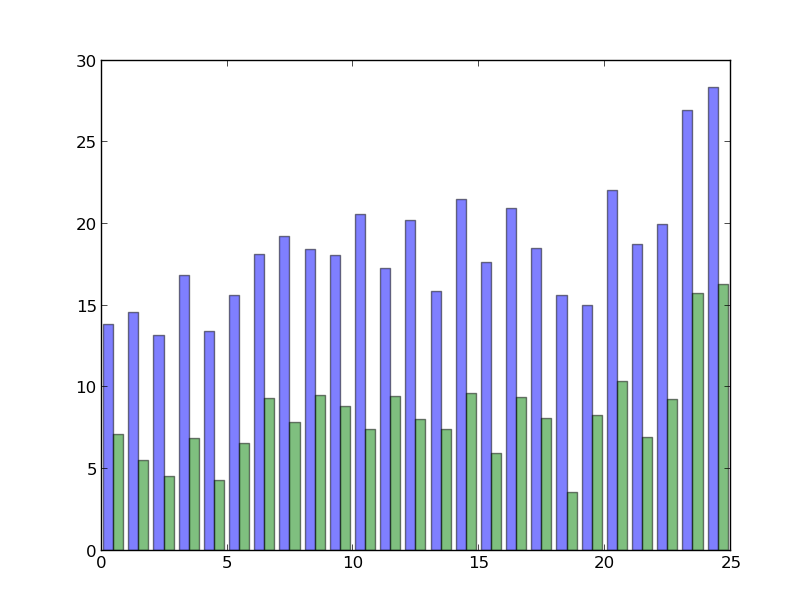
\includegraphics[width=5in]{tr-te-diff_FF-TT}}
\caption{Accuracy differential between training and test as a function of chord class, ordered along the x-axis from most to least common in the dataset for ETD:False (blue) and ETD:True (green) conditions.}
\label{fig:classes}
\end{figure}

One potential cause of over-fitting is due to an under-representation of some chord classes in the dataset.
If this were the case, we would see the most frequent classes unaffected by data augmentation, while less common classes would exhibit drastic swings in performance.
Focusing here on Arch:3--1, Figure \ref{fig:classes} shows the change in accuracy between data conditions for both training and test sets as a function of chord class, sorted by most to least common in the dataset.
This plot indicates that, while transposing data during training reduces over-fitting, it does so uniformly across chord classes, on the order of about $10\%$.
Therefore, all chord classes benefit equally from data augmentation, which is characteristic of intra-class variance more so than inadequate data for less common classes.

\begin{figure}[!t]
\centering
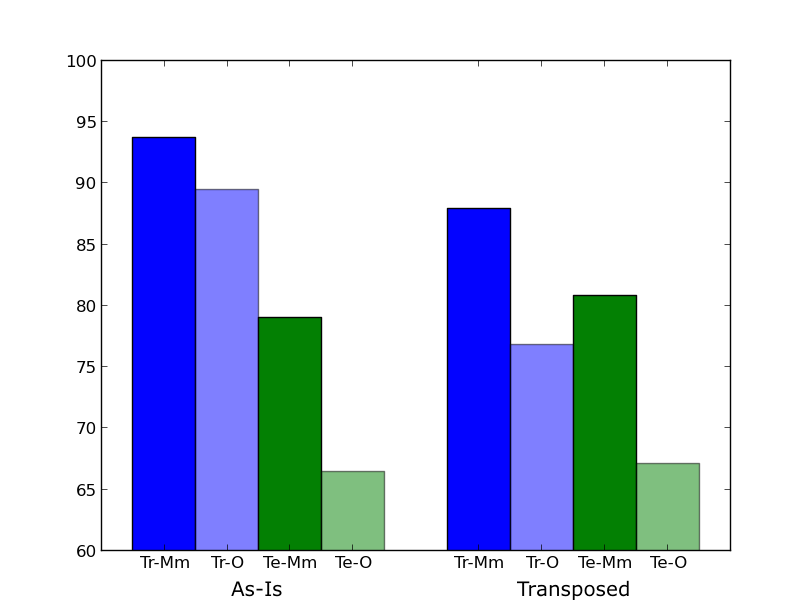
\includegraphics[width=5in]{FF-TT_Mm-vs-other}
\caption{Effects of transposition on recognition accuracy as a function explicitly labeled Major-Minor chords (dark bars), versus other chord types (lighter bars) that have been resolved to their nearest Major-Minor equivalent, for training (blue) and test (green) in standard (left) and transposed (right) conditions.}
\label{fig:strict_vs_others}
\end{figure}

If this is indeed the case, there are likely two main sources of intra-class variance: the practice of resolving all chord classes to Major-Minor, or error in the ground truth transcriptions.
As a means to assess the former, Figure \ref{fig:strict_vs_others} plots the accuracy for chords that strictly labeled root-position Major-minor (Mm) versus all other (O) chords that are mapped into these classes in the train (Tr) and test (Te) conditions, with and without transposition.
This is a far more informative figure, resulting in a few valuable insights.
First, there is a moderate drop in performance over the training set for strictly Major-minor chords when data are transposed ($\approx -5\%$), but this causes a noticeable increase in generalization for strictly Major-minor chords in test set ($\approx +3\%$).
Other chords, however, experience a significant decrease in performance within the training set ($\approx -11\%$) with transposition, but register a negligible improvement in the test set ($>1\%$).
One interpretation of this behavior is there is too much conceptual variation in the space of Other chords to meaningfully generalize to unseen data that is also not strictly Major-minor.
This defintion by exclusion gives rise to a class subset that is less populated than its strict counterpart, but will inherently contain a wider range of musical content.
Though a sufficiently complex model may be able to overfit these datapoints in the absence of transposition, counting each observation toward every pitch class distributes the added variance across all classes evenly.
This causes the model to ignore the most uncommon class ``modes'' as noise, while reinforcing the strict Major-minor model in the process.

% Additionally, not only is generalization for strict Major-minor chords considerably better than that of Other chords when trained with transposition, but it achieves better recall than Other chords in the training set.
% This means ...

\begin{figure}[!t]
\centering
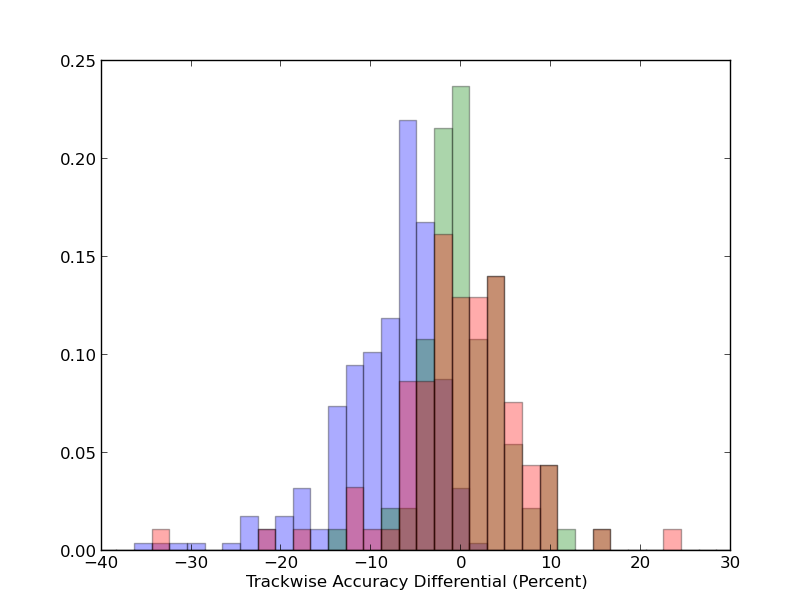
\includegraphics[width=5in]{arch_5-FF_TT_accdiff2}
\caption{Histograms of trackwise recall differential between normal and transposed data conditions, for training (blue), validation (red) and test (green) datasets.}
\label{fig:acc_diff}
\end{figure}

In addition to the effects of vocabulary resolution, there is also a question where this error resides in the data.
To address this point, we consider track-wise histograms of recall differential before and after transposing data for the training, validation, and test splits, shown in Figure \ref{fig:acc_diff}.
Interestingly, performance over most tracks is unaffected or only slightly changed by the transposed data condition, as evidenced by the near-zero mode of the distributions.
Some tracks in the training set, however, result in considerably worse performance when the data is transposed.
This is intuitively satisfying because the repetitive nature of music would cause observations drawn from the same recording to be highly correlated, and therefore multiple instances of rare chords, outliers, or labeling errors should be well localized.
Additionally, this clearly indicates that some tracks are particularly challenging or problematic, and may offer insight into future areas of improvement.

\begin{figure}[!t]
\centering
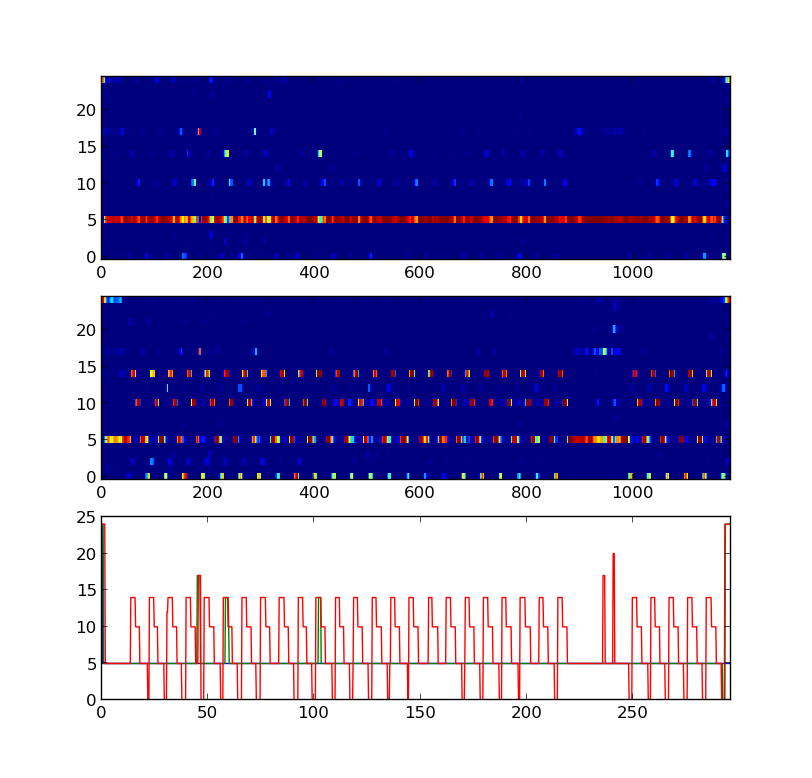
\includegraphics[width=5in]{u2-ff_tt_gtplot}
\caption{.}
\label{fig:u2fu}
\end{figure}

An instance of one such ``problem'' track, ``With or Without You'' by U2, is given in Figure \ref{fig:u2fu}.
Here, the ground truth transcription consists primarily of four chords: \texttt{D:maj}, \texttt{D:maj/5}, \texttt{D:maj6/6}, and \texttt{D:maj(4)/4}.
When resolved to the Major-minor vocabulary, the transcription is reduced entirely to \texttt{D:maj}.
Without transposing data during training, the model is able to call nearly the entire track \texttt{D:maj}; with transposition during training, however, the model is unable to reproduce the ground truth transcription and instead tracks the bass motion, producing \texttt{D:maj}, \texttt{A:maj}, \texttt{B:min}, and \texttt{G:maj}, a very common harmonic progression in popular music.
As far as quantitative evaluation is concerned, this second estimation exhibits a high degree of mismatch with the reference transcription, but is qualitatively reasonable and arguably far more useful to a musician.

\subsection{Conclusions}
\label{subsec:conclusions}

Following this initial inquiry, there are a number of conclusions to draw that should influence subsequent work.
First and foremost, the practice of chord name resolution is the largest source of error, both in training and test, as doing so creates multi-modal distributions that can be difficult to model directly.
This challenge stems from the combination of weak conceptual associations between the classes, and diminshed amount of data for the model to discover such diverse relationships.
Therefore, if for this reason alone, future work should consider larger vocabulary chord estimation, as the additional labeling information simplifies the learning problem by encouraging the machine to model different pockets of class densities separately.
Additionally, there is some evidence, in the vein of Figures \ref{fig:acc_diff} and \ref{fig:u2fu}, that chord names with modified intervals or bass information may be used inconsistently across transcriptions.
The tracks that are most affected through the use of transpostion during training are those consisting of non-standard spellings.
Seeing as how such instances comprise a relatively small portion of the data, ignoring these over-specified chord names should lead to more stable evaluation while maximizing confidence in the ground truth annotations.


\section{Large Vocabulary Chord Estimation}
\label{subsec:large_vocabulary_ace}

In light of observations resulting from the previous study, combined with other recent trends in ACE research, we now focus on the task of large vocabulary ACE.
As mentioned, there is a smaller subset of research focusing on vocabularies past the Major-minor formulation, but, for the same reasons discussed in \ref{subsec:problem_formulation}, comparing these efforts directly is problematic due to differences in vocabularies considered and the data used.
One of the most advanced automatic chord estimation systems to date is the recent work of Cho \cite{Cho2014}.
Not only is this work one of the highest performing systems at the recent iteration of MIReX, but we are also priviledged by access to a software implementation, thereby enabling direct comparisons with other work.
It also considers a significantly larger vocabulary than previous work, and presents an even greater challenge to the application of deep learning to ACE.


\subsection{Data Considerations}
\label{subsec:data_considerations}
% Say something about Taemin's dissertation.
Following the previous work of Cho \cite{Cho2014}, we consider thirteen chord qualities, given in Table \ref{tab:qualities} in all 12 pitch classes, plus one no-chord class, for a total of 157 classes.
Having all four datasets at our disposal, we merge these information sources into the largest collection of chord transcriptions used to date, totalling 1235 tracks.
After performing fuzzy string matching on a manifest of the known artist names and track titles, we identify X redundant tracks and randomly drop all but one from the collection; this results in a final count of 12XX tracks.

Combining conclusions from the previous section with recent discussion of evaluation at MIReX, we chose to ignore all chord instances with names that specify interval modifications, e.g. \texttt{A:min(*b3)}, or bass scale degrees that are not strictly contained by the chord shorthand, e.g. \texttt{C:maj/4}.
The decision is made in the interest of annotation consistency; considering that the cumulative data is compiled from multiple sources and several dozen annotators, it is quite unlikely that such conventions were applied identically by all subjects involved.
This subset comprises only a small percentage of the overall data ($?.?\%$), and helps filter out curious chord spellings, such as \texttt{D:maj(\*1)/$\sharp$1} or \texttt{A:maj(2,\*3)/2}.

% Statistics
Unsurprisingly, as the data is collected from real music, the distribution of absolute chord classes is extremely imbalanced.
In fact, some chord qualities do not occur in every root, and stratifying the data for training, validation, and testing only exacerbates the issue.
Much previous work, including the previous discussion, has demonstrated that chord names can be rotated to distribute instances across qualities, rather than absolute classes, motivating root-invariant analysis.
A root-invariant histogram of the chord qualities contained in the merged dataset, given in Figure \ref{fig:training_distribution}, clearly shows there is severe relative and absolute class imbalance.
To the former, a stark division exists between the majority classes (\texttt{maj}, \texttt{min}, \texttt{maj7}, \texttt{min7}, \texttt{7}, and \texttt{N}), and the minority classes (\texttt{maj6}, \texttt{min6}, \texttt{dim}, \texttt{aug}, \texttt{sus4}, \texttt{sus2}, \texttt{dim7}, \texttt{hdim7}).
The ratio, for example, between the most and least common qualities, \texttt{maj} and \texttt{dim7} respectively, is nearly three orders of magnitude ($\approx 700$).
Arguably, the more challenging imbalance is an overall lack of data for some minority classes.
Over all roots, the total duration of \texttt{dim7} is on the order of hundreds of seconds.
Considering the repetitive structure of music, it is reasonable to assume that these few instances also occur in the same small number of tracks, limiting the variability of this data.


\subsection{Research Questions}
\label{subsec:research_questions}

What can we do to overcome these issues of class imbalance?
% Build class invariance into the model
% use dropout during training
% smaller inputs, more constraints, leverage HMM for context / stabilization
How does the deep learning system compare to the state of the art?
% Beats it! depending on who you ask, at least
What are the advantages and challenges of training with larger vocabularies?
% Resolve predictions back to maj / min, how does it do? Should be better...
% Larger vocabularies result in more class collisions
% But this is actually a manifestation of ambiguity



\subsection{Experimental Setup}

This work proceeds directly from the previous study, and takes a similar approach in many facets.
There are a handful of important distinctions to make between the two, however, and these differences are detailed here.

\subsubsection{}

A comparable constant-Q transform is applied to the audio at a framerate of 20Hz, without subsequent low-pass filtering or decimation, and time-frequency patches are formed from 20 frames, corresponding to 1 second.
Whereas the previous study aimed to learn context directly, there is the inherent concern that a low input framerate will reduce the amount of data available for training beyond what is required by the model.
In lieu of learning this context, standard post-filtering will be applied in the form of a uniform-transition HMM with a tunable self-transition penalty, consistent with \cite{Cho2014PhD}.

Additionally, local contrast normalization is included as a standard preprocessing stage, with minor modifications.
In previous work, a threshold is placed on the scaling term given by the average standard deviation over the entire input.
While this may be suitable in the field of computer vision, where spatial dimensions are equivalent in 2-space, audio data behave differently in time and frequency.
Namely, complex sounds often exhibit an overtone series, and energy becomes more densely concentrated in higher frequencies.
This can have the undesirable effect of inadequately gaining regions that are more sparse.
To correct for this behavior, the scaling coefficient is adjusted such that the frequency range considered is a piecewise function of frequency height, defined as follows:

\begin{equation}
X_filt = (X \circledast W) \\
V = X_filt - X \\
S_k = V \circledast W_k \\
S_k = max(S_k, \mu_{S_k})
Y = \sum_{k=0}^{K-1} g_k * \frac{V}{S_k}
\end{equation}

\noindent To illustrate the benefit of this piecewise combination, an example track is given in Figure \ref{lcn_mods}, both with and without the octave-dependent modification.

\begin{figure}[!t]
\centering
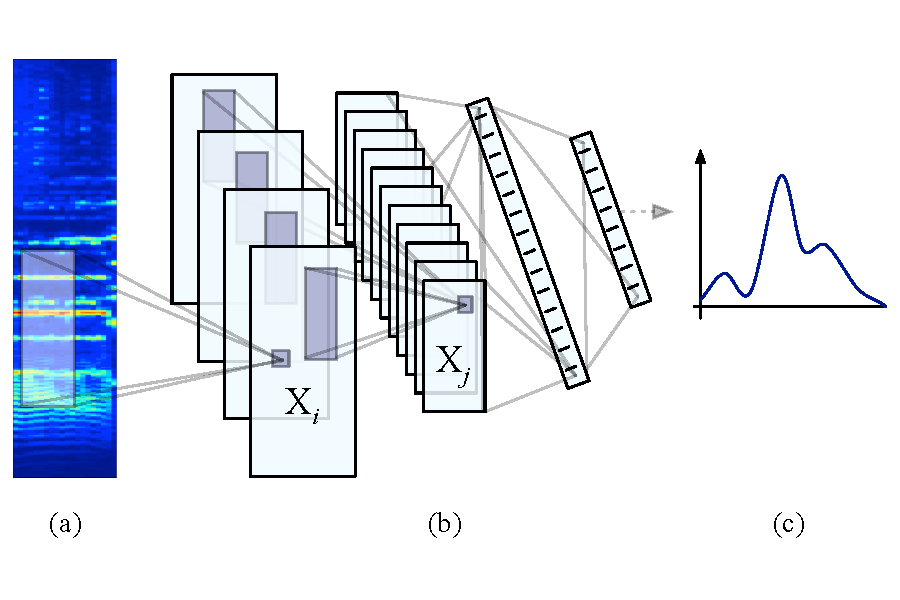
\includegraphics[width=3in]{pitch-CNN-prob}
\caption{The visible effects of octave-dependent LCN, before (top) and after (bottom).}
\label{fig:lcn_mods}
\end{figure}


\subsubsection{Designing a Root-Invariant Classifier}

One of the key findings from the previous study of deep networks for ACE, consistent with previous research, is the importance of enforcing or encouraging root-invariance in the model.
With GMMs, this is typically achieved by rotating all data, i.e. chroma features, to the same root and fitting a model for each quality.
Then, when applying the model, likelihoods are estimated for each root by circularly rotating chroma through all twelve positions to recover the full space of chord classes.
In our previous work on chord recognition, this concept was mimicked by rotating the data in the input domain.
While it led to improved results, rotating the data is less than ideal for at least two reasons.
One, it is an implicit, rather than explicit, association between classes, and the model is tasked with learning these redundant relationships.
In the case of chord recognition, the model needs to learn the same behavior 12 times over, to represent each quality in every root.
Two, rotating data in the input space may create unnatural artifacts in the kinds of data the model learns to expect, and it is not clear what, if any, side effects this may have.
It is assumed that this does not fundamentally change the latent distribution of the data used for training, but it may cause a mismatch with real data at test time.

An alternative to rotating the data, as convolutional networks have amply demonstrated, is to build the invariance directly into the architecture.
This is realized here by defining a fully convolutional model, such that the classifier's weights for each quality are shared over all roots; a diagram of this configuration is given in Figure \ref{fig:fullconvnet}.
Simplifying conceptually, this proceeds as follows: the penultimate representation is designed to yield a matrix with shape $(12 \times N)$, corresponding to the number of pitch classes and the chosen output dimensionality of the second to last layer, respectively; the chord classifier is then applied by taking the inner product with a weight matrix with shape $(N \times 13)$, corresponding to the dimensionality of the previous layer and the number of chord qualities, respectively.
For ease and efficiency this is implemented as a convolution, but the result is equivalent.
This produces a $(12 \times 13)$ matrix, which is flattened to represent the 13 qualities in all possible roots.
The no-chord condition is not captured by this operation, however, and a separate fully connected layer is applied in parallel to the flattened penultimate representation to estimate this class independently, which is then concatenated to the chord estimator.
Finally, this combined representation of 157 classes is normalized by the softmax operation, producing a probability mass function over all classes.

\begin{figure}[!t]
\centering
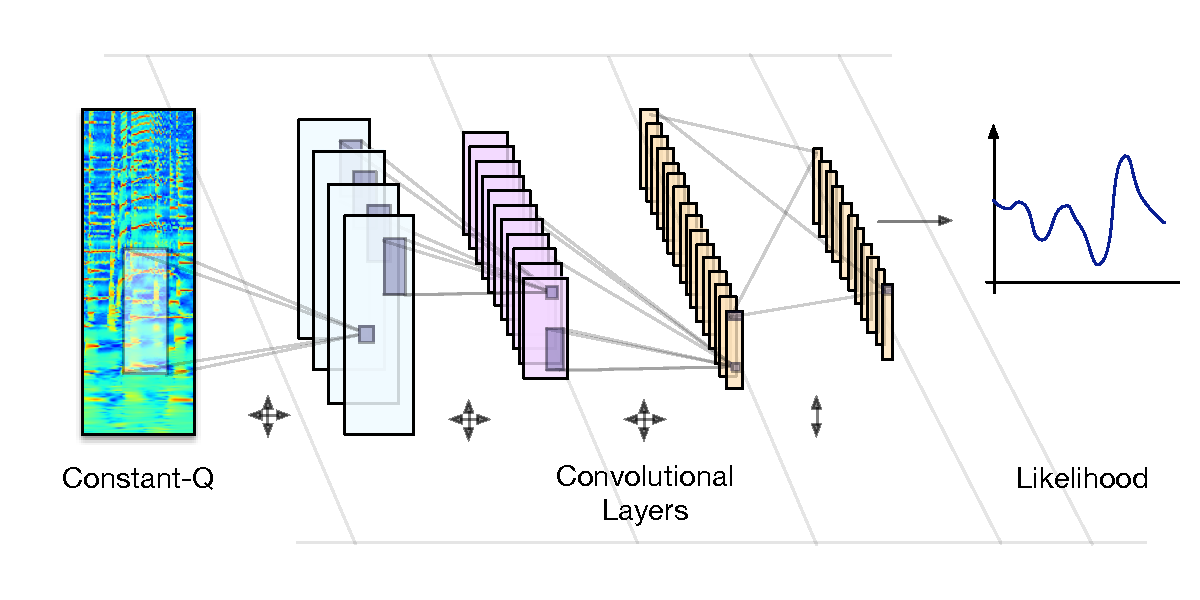
\includegraphics[width=5in]{fullconvnet}
\caption{A Fully Convolutional Chord Estimation Architecture.}
\label{fig:fullconvnet}
\end{figure}



\subsubsection{Correcting Bias via Likelihood Scaling}

Take the data as-is, optimize the negative log-likelihood over the dataset.

$L(X^i, Y^i) = -ln(\mathcal{L}(X^i|Y^i))$

Then, at test time, apply likelihood scaling.
Consistent with ASR and other imbalanced learning problems.
Appropriately suited to HMM processing now


\subsubsection{Convolutional Dropout}
Here, we extend the principles of dropout, discussed in Chapter \ref{chp:deep_learning}, to 3D convolutions.
In the weight-matrix case, training with dropout effectively ignores activations of an transformed output, setting them to zero.
Considering each output coefficient as a measure of activation for a given ``feature'', the act of dropout can be interpretted as sub-sampling the feature extractors learned by the model.

By extension, there are two ways the same principle could be applied in the case of 3D convolutions.
One, the $i^{th}$ kernel, $W_i$, can be masked with probability $p$, resulting in the possibly empty feature map, $Z_i$:

\begin{equation}
Z_i = binomial(p) * h(X \circledast W_i + b_i) / (1.0 - p)
\end{equation}

\noindent where the output is also scaled by the complement of the probability.
Here, it is expected that each kernel learns a collection of feature extractors that, on average, work well together.
In the language of coadaptation, the tensor can be seen as a ``team'' of feature detectors, and as such correlations are broken up at this mid, as opposed to global, level.

Alternatively,



\subsection{Experimental Setup}


TODO: Observe that it learns a root invariant representation of qualities
Distance matrix between qualities
Ave vectors for same qualities in different roots



We need to develop better means of curating datasets such that objective measures better correspond with subjective experience.
